\begin{table}[H]
    {\renewcommand{\arraystretch}{1.2}%
    \setlength{\tabcolsep}{0.3em}%
\begin{tabular}{bababab}
\toprule

\rowcolor{white} \null &
\textbf{Synthetic$_{\mathbf{\mathcal{F}}}$} & \textbf{Synthetic$_{\mathbf{\mathcal{\beta}}}$} &
\textbf{Lehrpfad$_{\mathbf{\mathcal{F}}}$} & \textbf{Lehrpfad$_{\mathbf{\mathcal{\beta}}}$} &
\textbf{Office$_{\mathbf{\mathcal{F}}}$} & \textbf{Office$_{\mathbf{\mathcal{\beta}}}$} \\
\midrule

\rowcolor{lightgray}
\textbf{Keypoint Count} &
    \num{49469} & \num{45811} &
    \num{165916} & \num{159291} &
    \num{13417} & \num{12370} \\
\textbf{Correspondences} &
    \num{18593} & \num{16139} &
    \num{11023} & \num{6542} &
    \num{2303} & \num{872} \\
\rowcolor{lightgray}
\textbf{True Positives} &
    \num{11724} & \num{10039} &
    \num{4018} & \num{1370} &
    \num{1547} & \num{431} \\
\textbf{False Positives} &
    \num{10993} & \num{10520} &
    \num{53693} & \num{59940} &
    \num{3418} & \num{4215} \\
\rowcolor{lightgray}
\textbf{False Negatives} &
    \num{6869} & \num{6100} &
    \num{7005} & \num{5172} &
    \num{756} & \num{441} \\

\bottomrule
\end{tabular}

    }
    \caption[Keypoint and matching results for \texttt{\acrshort{orb}/raw/default}]{\emph{Keypoint and matching results for \texttt{\acrshort{orb}/raw/default}.} The high number of false negatives and the low Youden index are an indicator for problems of the algorithm. The amount of additional keypoints for \glspl{flexion-image} is lower than for \acrshort{sift}.}
\end{table}
\acrshort{orb}'s detector finds less keypoints than \acrshort{sift} for both \glspl{flexion-image} and \glspl{bearing-angle-image}.
But their size, response and location distribution (Appendix~\ref{sec:orb_stats}) indicate severe problems.
Keypoints are not detected over multiple scales and the response shows a very inconsistent pattern over the different datasets.
For \emph{Lehrpfad} the keypoints cluster in the middle and the borders of the field-of-view of the depth sensors.
Those regions contains sharp edges from feature image to black because of missing range data.
The \acrshort{fast} keypoint detector characteristics of comparing brightness values at different sampling points is to blame for the keypoints bad performance.
Similar to \acrshort{surf}'s shortcoming, it does not deal well with the smoother gray changes but requires sharp edges.
As \acrshort{orb} employs blurring and scale space, too, the effect of missing contrast between sampling points worsens in higher levels of the pyramid, yielding no keypoints there.
\begin{figure}[htp]
\begin{subfigure}[t]{0.45\linewidth}
    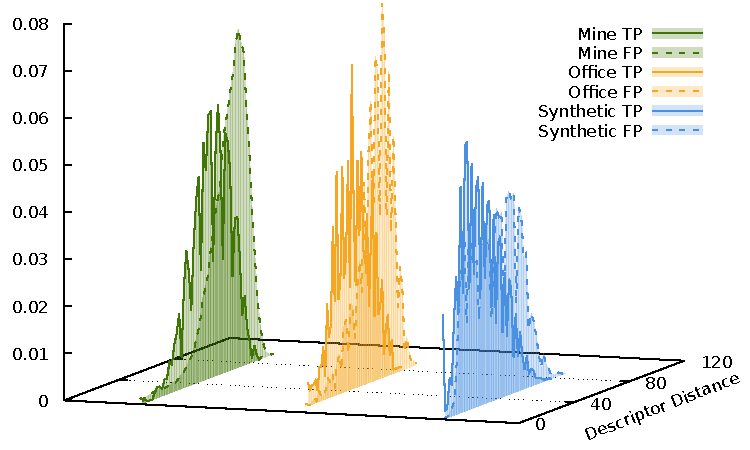
\includegraphics[width=\linewidth]{chapter06/results/ORB/flexion/descriptor_distances.pdf}%
    \caption{\gls{flexion-image}}
\end{subfigure}\quad
\begin{subfigure}[t]{0.45\linewidth}
    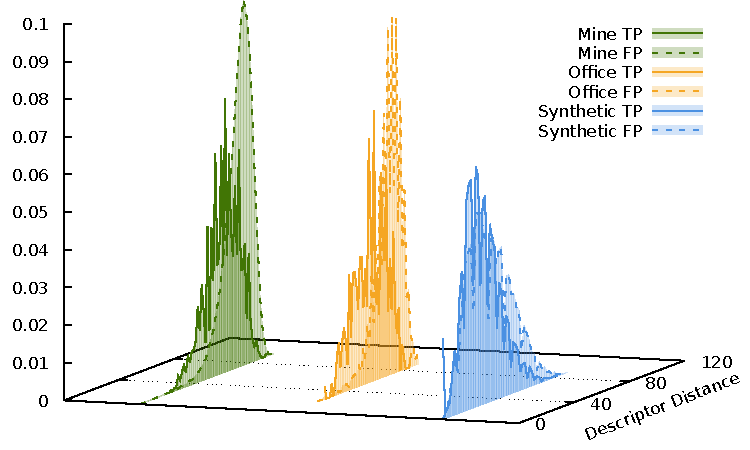
\includegraphics[width=\linewidth]{chapter06/results/ORB/bearing/descriptor_distances.pdf}%
    \caption{\gls{bearing-angle-image}}
\end{subfigure}
\caption[\acrshort{orb} descriptor distances]{\emph{\acrshort{orb} descriptor distances.} The results show a slight separation of true positive from false positives. The binary descriptor compares brightness values on specific sampling points. This mechanism is different from \acrshort{sift} or \acrshort{surf} and seemingly not as robust as \acrshort{sift}.}\label{fig:orb_descriptor_distances}
\end{figure}
The descriptor distance in Figure~\ref{fig:orb_descriptor_distances} show some separation between true positives and false positives better than \acrshort{surf} but worse than \acrshort{sift}.
In \acrshort{ROC} space (Figure~\ref{fig:orb_roc}) these mixed result show in random performance for \emph{Lehrpfad} and OK performance for \emph{Synthetic} and \emph{Office}.
Everything considered, \acrshort{orb} is not suitable for the proposed feature images.
\begin{figure}[htp]
\begin{subfigure}[t]{0.45\linewidth}
    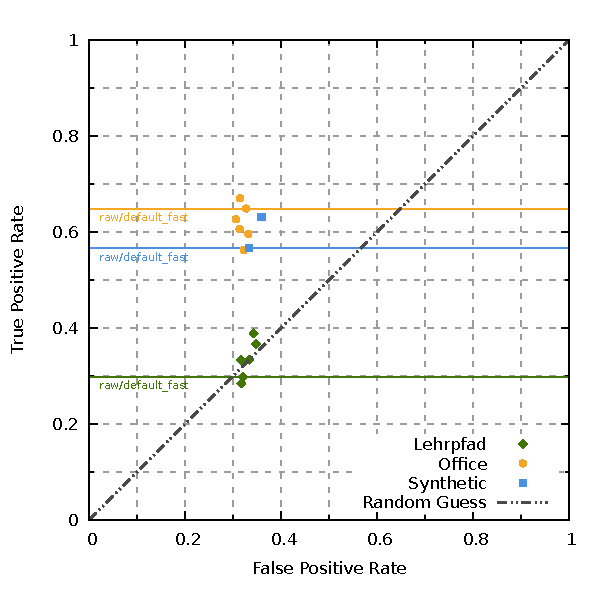
\includegraphics[width=\linewidth]{chapter06/results/ORB/flexion/roc.pdf}%
    \caption{\gls{flexion-image}}
\end{subfigure}\quad
\begin{subfigure}[t]{0.45\linewidth}
    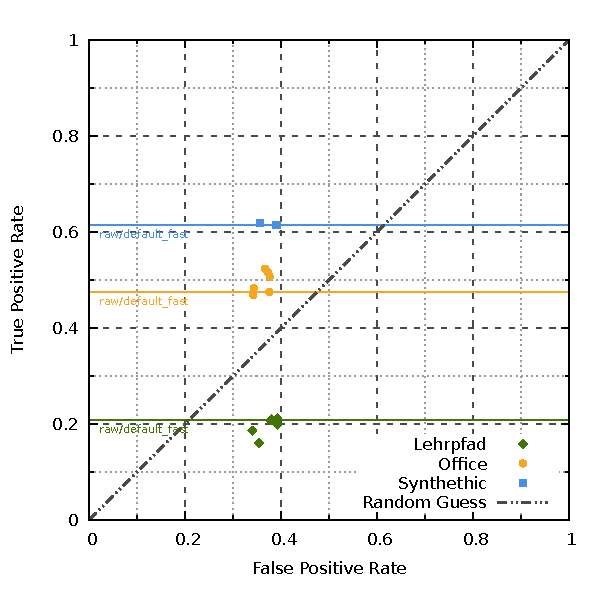
\includegraphics[width=\linewidth]{chapter06/results/ORB/bearing/roc.pdf}
    \caption{\gls{bearing-angle-image}}
\end{subfigure}
\caption[\acrshort{ROC} graphs for \acrshort{orb}]{\emph{\acrshort{ROC} graphs for \acrshort{orb}.} The results for \acrshort{orb} are mixed in the \acrshort{ROC} graph. It can not be rejected based on their findings, but additional characteristics of the keypoints and their distribution are more important factors for this decision.}\label{fig:orb_roc}
\end{figure}
